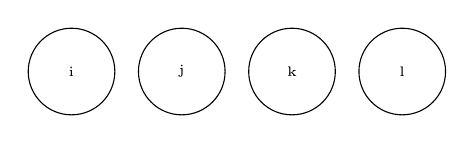
\begin{tikzpicture}
    \def\d{1.4}
    \def\size{1.1}
    \node(c1) [circle, draw, minimum size = \size cm] at (\d * 0,0) {\tiny i};
    \node(c2) [circle, draw, minimum size = \size cm] at (\d * 1,0) {\tiny j};
    \node(c3) [circle, draw, minimum size = \size cm] at (\d * 2,0) {\tiny k};
    \node(c4) [circle, draw, minimum size = \size cm] at (\d * 3,0) {\tiny l};
\end{tikzpicture}